\section{Cài đặt, Biên dịch và Hướng phát triển}

\subsection{Yêu cầu hệ thống}

\begin{itemize}
    \item \textbf{Hệ điều hành}: Windows 10 hoặc 11. Console của các phiên bản này hỗ trợ mã điều khiển ANSI, cần để tô màu khối và vẽ đè khung hình.
    \item \textbf{Trình biên dịch}: G++ bản MinGW-w64 hỗ trợ C++11 (phiên bản 4.8.1 trở lên), hoặc Microsoft Visual C++ từ Visual Studio 2015 trở lên.
    \item \textbf{Cửa sổ dòng lệnh}: Command Prompt, PowerShell hoặc Windows Terminal (khuyến nghị, vì hiển thị tốt ký tự Unicode). Kích thước tối thiểu khoảng 50 cột $\times$ 22 dòng.
\end{itemize}

\subsection{Hướng dẫn biên dịch và Chạy chương trình}

Mã nguồn chỉ có một tệp \texttt{tetris/main.cpp} và không phụ thuộc thư viện ngoài. Chỉ cần biên dịch một lần ra tệp \texttt{.exe}, sau đó có thể chép tệp này sang máy Windows khác để chạy (Hình~\ref{fig:quy_trinh_trien_khai}).

\begin{figure}[H]
    \centering
    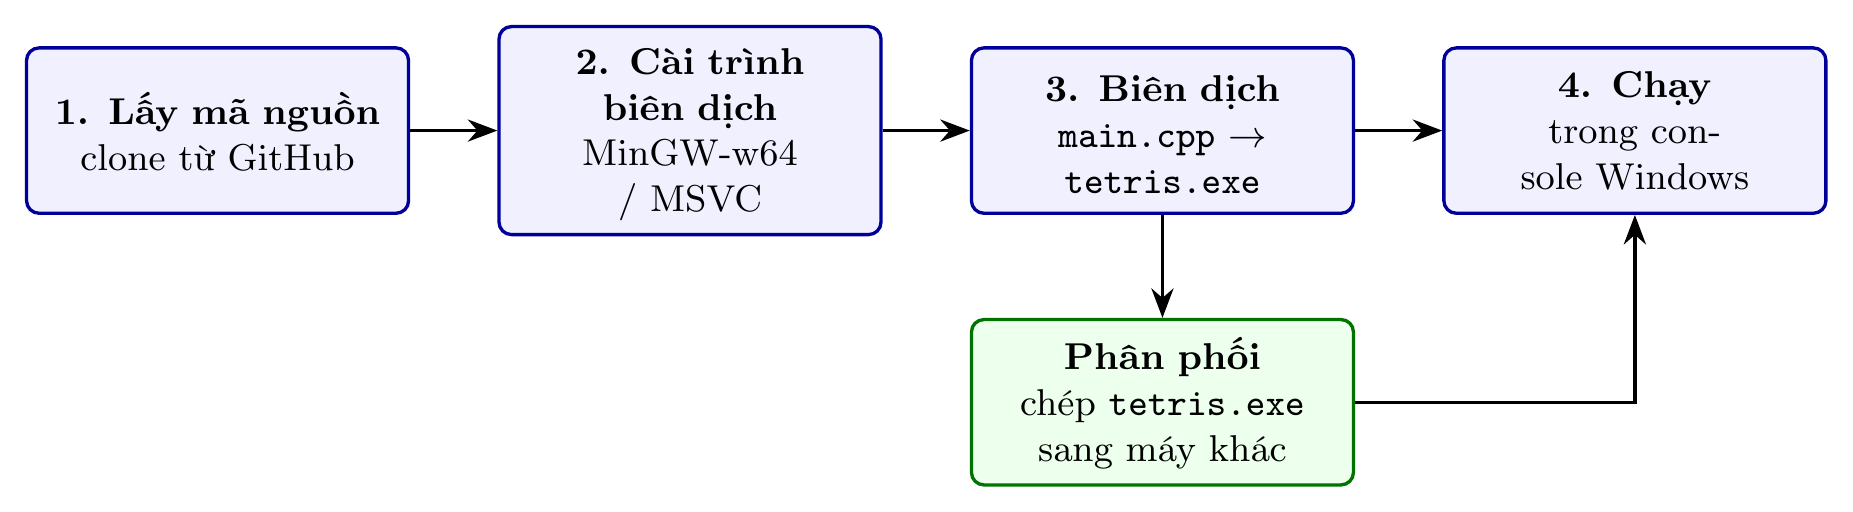
\includegraphics[width=0.85\textwidth]{04_tai_lieu_ky_thuat/so_do/trien_khai.png}
    \caption{Quy trình biên dịch và triển khai trò chơi}
    \label{fig:quy_trinh_trien_khai}
\end{figure}

\subsubsection{Cách 1: Dùng G++ (MinGW-w64)}

\begin{enumerate}
    \item Cài MinGW-w64 (qua MSYS2 hoặc gói WinLibs) và thêm thư mục \texttt{bin} của nó vào biến môi trường \texttt{PATH}. Gõ \texttt{g++ --version} để kiểm tra.
    \item Lấy mã nguồn, biên dịch và chạy:
\begin{lstlisting}[language=bash, caption={Lấy mã nguồn, biên dịch và chạy bằng g++}]
git clone https://github.com/26730046/Tetris.git
cd Tetris
g++ -std=c++11 -O2 tetris/main.cpp -o tetris.exe
.\tetris.exe
\end{lstlisting}
    \item Nếu muốn chép tệp \texttt{.exe} sang máy chưa cài MinGW, thêm tùy chọn \texttt{-static} khi biên dịch. Nếu không, máy đích có thể báo thiếu tệp \texttt{.dll}.
\end{enumerate}

\subsubsection{Cách 2: Dùng Visual Studio (MSVC)}

\begin{enumerate}
    \item Tạo dự án \textit{Console App} (C++), rồi thay tệp mẫu bằng \texttt{tetris/main.cpp}.
    \item Thêm tùy chọn \texttt{/utf-8} (\textit{Project Properties} $\rightarrow$ \textit{C/C++} $\rightarrow$ \textit{Command Line}) để chuỗi tiếng Việt không bị lỗi phông.
    \item MSVC báo lỗi C4996 với các hàm nhận phím của \texttt{<conio.h>} vì coi chúng là đã lỗi thời. Để khắc phục, tắt \textit{SDL checks} hoặc thêm macro \texttt{\_CRT\_NONSTDC\_NO\_DEPRECATE}.
    \item Chọn cấu hình \textit{Release} và nhấn \textit{Ctrl + F5}.
\end{enumerate}

\subsubsection{Một số lỗi thường gặp}

\begin{table}[H]
    \centering
    \caption{Một số lỗi thường gặp và cách khắc phục}
    \label{tab:loi_thuong_gap}
    \renewcommand{\arraystretch}{1.3}
    \begin{tabularx}{\textwidth}{|p{5.4cm}|X|}
        \hline
        \textbf{Hiện tượng} & \textbf{Nguyên nhân và cách khắc phục} \\
        \hline
        Lỗi không nhận \texttt{nullptr}, \texttt{override} & Trình biên dịch đang dùng chuẩn cũ. Thêm \texttt{-std=c++11}. \\
        \hline
        Không tìm thấy \texttt{conio.h}, \texttt{windows.h} & Đang biên dịch trên Linux/macOS, nơi chương trình chưa được hỗ trợ. \\
        \hline
        Màn hình hiện chuỗi lạ như \texttt{[96m} & Console không hỗ trợ mã ANSI. Dùng Windows 10 trở lên hoặc Windows Terminal. \\
        \hline
        Bấm phím không có tác dụng & Đang bật Caps Lock. Trò chơi chỉ nhận phím chữ thường. \\
        \hline
    \end{tabularx}
\end{table}

\subsection{Đánh giá hiệu năng và Hạn chế hiện tại}
% [Gợi ý nội dung: Đánh giá độ mượt của màn hình (hạn chế hiện tượng nhấp nháy do system("cls")), độ trễ khi nhận phím, tính tương thích đa nền tảng]
\textit{[Nội dung bổ sung sau: Đánh giá hiệu năng và các điểm hạn chế cần khắc phục]}

\subsection{Hướng mở rộng và Phát triển trong tương lai}
% [Gợi ý nội dung: Tích hợp thư viện đồ họa (SFML, SDL2, Raylib), thêm hiệu ứng âm thanh, lưu trữ điểm cao (High Score File I/O), chế độ chơi 2 người (Multiplayer)]
\textit{[Nội dung bổ sung sau: Kế hoạch mở rộng tính năng và nâng cấp đồ họa]}
